\documentclass[aspectratio=169]{beamer}

% ---------- Theme & Colours ----------
\usetheme{Madrid}
\usecolortheme{default}

\definecolor{NavyBlue}{RGB}{31,56,137}
\definecolor{LightBlue}{RGB}{173,198,230}
\definecolor{DarkBlue}{RGB}{20,40,100}
\definecolor{AlertRed}{RGB}{180,30,30}
\definecolor{GreenOK}{RGB}{30,140,60}
\definecolor{CarRed}{RGB}{220,50,50}
\definecolor{CarOrange}{RGB}{230,130,30}
\definecolor{CarGreen}{RGB}{50,160,50}
\definecolor{CarBlue}{RGB}{65, 105, 225}
\definecolor{CarGray}{RGB}{150,150,150}

\setbeamercolor{palette primary}{bg=NavyBlue,fg=white}
\setbeamercolor{palette secondary}{bg=DarkBlue,fg=white}
\setbeamercolor{palette tertiary}{bg=NavyBlue,fg=white}
\setbeamercolor{palette quaternary}{bg=DarkBlue,fg=white}
\setbeamercolor{structure}{fg=NavyBlue}
\setbeamercolor{section in toc}{fg=NavyBlue}
\setbeamercolor{block title}{bg=NavyBlue,fg=white}
\setbeamercolor{block body}{bg=LightBlue!25,fg=black}
\setbeamercolor{alerted text}{fg=AlertRed}
\setbeamercolor{frametitle}{bg=NavyBlue,fg=white}
\setbeamercolor{title}{fg=white,bg=NavyBlue}
\setbeamerfont{frametitle}{size=\large,series=\bfseries}

% ---------- Packages ----------
\usepackage{tikz}
\usetikzlibrary{arrows.meta, shapes.geometric, shapes.callouts, positioning, decorations.pathreplacing, calc}
\usepackage{amsmath, amssymb}
\usepackage{booktabs}
\usepackage{xcolor}
\usepackage{ifthen}

% ---------- Footer ----------
\setbeamertemplate{footline}{%
  \leavevmode%
  \hbox{%
    \begin{beamercolorbox}[wd=.333\paperwidth,ht=2.25ex,dp=1ex,center]{palette secondary}%
      \usebeamerfont{author in head/foot}\insertshortauthor
    \end{beamercolorbox}%
    \begin{beamercolorbox}[wd=.334\paperwidth,ht=2.25ex,dp=1ex,center]{palette primary}%
      \usebeamerfont{title in head/foot}\insertshorttitle
    \end{beamercolorbox}%
    \begin{beamercolorbox}[wd=.333\paperwidth,ht=2.25ex,dp=1ex,right]{palette secondary}%
      \usebeamerfont{date in head/foot}\insertshortdate{}\hspace*{2em}
      \insertframenumber{} / \inserttotalframenumber\hspace*{2ex}
    \end{beamercolorbox}}%
  \vskip0pt%
}
\setbeamertemplate{navigation symbols}{}

% ---------- Title Info ----------
\title[MOEA/D]{Multi-Objective Evolutionary Algorithms based on Decomposition (MOEA/D)}
\author[Islam, Mobin, Nabi]{Md.\ Rashidul Islam \and Fathum Mobin \and Md.\ Riyadun Nabi}
\date[February 2026]{23 February 2026}

% ============================================================
\begin{document}
% ============================================================

%% ---- Title Slide ----
\begin{frame}
  \titlepage
\end{frame}

% %% ============================================================
% %% HOOK SLIDE — Insert immediately AFTER \titlepage frame
% %%              and BEFORE the "What Will You Learn Today?" frame
% %% ============================================================

% \begin{frame}[plain]
% \begin{center}

% % ---------------- STEP 1 ----------------
% \onslide<1->{
% \vspace{1.8em}
% {\large\color{NavyBlue!60} Today We will talk about}\\[0.8em]

% {\fontsize{32}{36}\selectfont\bfseries\color{NavyBlue}
% MOEA/D}\\[0.5em]

% {\normalsize\color{DarkBlue}
% \textbf{M}ulti-\textbf{O}bjective
% \textbf{E}volutionary
% \textbf{A}lgorithm
% by
% \textbf{D}ecomposition}
% }

% \vspace{1.2em}

% % ---------------- STEP 2 ----------------
% \onslide<2->{
% \begin{tikzpicture}
% \node[draw=NavyBlue!30, fill=NavyBlue!6, rounded corners=8pt,
%       font=\normalsize, inner sep=14pt, text width=8.5cm, text centered]
%   {A powerful \textbf{evolutionary algorithm}\\
%    for solving \textbf{multi-objective optimization} problems.};
% \end{tikzpicture}
% }

% \vspace{1.6em}

% % ---------------- STEP 3 — PIVOT ----------------
% \onslide<3->{
% {\large\color{NavyBlue!70}
% But before we understand the algorithm...}
% }

% \vspace{0.8em}

% \onslide<4->{
% \begin{tikzpicture}
% \node[draw=NavyBlue, fill=NavyBlue!10, rounded corners=10pt,
%       font=\large\bfseries, inner sep=18pt, text width=8.0cm,
%       text centered, text=NavyBlue]
%   {we must understand the \emph{problem}.};
% \end{tikzpicture}
% }

% \end{center}
% \end{frame}

%% ============================================================
%% HOOK SLIDE 1 — Big acronym reveal on dark background
%% ============================================================
{
\setbeamertemplate{footline}{}
\setbeamercolor{palette primary}{bg=DarkBlue,fg=DarkBlue}
\setbeamercolor{palette secondary}{bg=DarkBlue,fg=DarkBlue}
\setbeamercolor{palette tertiary}{bg=DarkBlue,fg=DarkBlue}
\setbeamercolor{palette quaternary}{bg=DarkBlue,fg=DarkBlue}
\setbeamertemplate{background}{%
  
\begin{tikzpicture}
    \useasboundingbox (0,0) rectangle (\paperwidth,\paperheight);
    \fill[DarkBlue] (0,-1cm) rectangle (\paperwidth,\paperheight);
    \fill[NavyBlue] (0,\paperheight-0.55cm) rectangle (\paperwidth,\paperheight);
  \end{tikzpicture}%
}
\begin{frame}[plain]

\begin{center}
\vspace{0.6em}
{\color{LightBlue!70}\footnotesize\bfseries\MakeUppercase{Today we will talk about}}

\vspace{1.0em}

{\fontsize{72}{76}\selectfont\bfseries\color{white}
MOEA/D}

\vspace{0.5em}

\onslide<1->{
{\color{LightBlue!80}\normalsize
\textbf{\color{white}M}ulti-\textbf{\color{white}O}bjective\ %
\textbf{\color{white}E}volutionary\ %
\textbf{\color{white}A}lgorithm based on \textbf{\color{white}D}ecomposition}
}

\vspace{1.4em}

\onslide<2->{
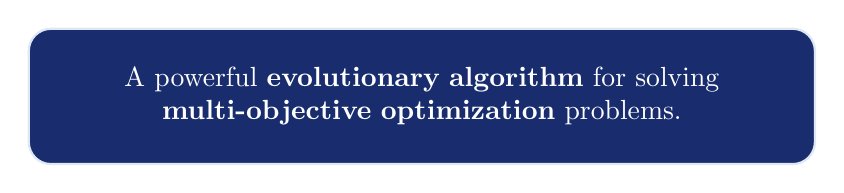
\begin{tikzpicture}
\node[draw=LightBlue!40, fill=NavyBlue!80!black, rounded corners=8pt,
      font=\normalsize\color{white}, inner sep=14pt, text width=9.0cm,
      text centered, line width=0.8pt]
  {A powerful \textbf{evolutionary algorithm} for solving\\
   \textbf{multi-objective optimization} problems.};
\end{tikzpicture}
}
\end{center}
\end{frame}
}

%% ============================================================
%% HOOK SLIDE 2 — Dramatic pivot: "But first… the PROBLEM"
%% ============================================================
{
\setbeamertemplate{footline}{}
\setbeamercolor{palette primary}{bg=DarkBlue,fg=DarkBlue}
\setbeamercolor{palette secondary}{bg=DarkBlue,fg=DarkBlue}
\setbeamercolor{palette tertiary}{bg=DarkBlue,fg=DarkBlue}
\setbeamercolor{palette quaternary}{bg=DarkBlue,fg=DarkBlue}
\setbeamertemplate{background}{%
  
\begin{tikzpicture}
    \useasboundingbox (0,0) rectangle (\paperwidth,\paperheight);
    \fill[DarkBlue] (0,-1cm) rectangle (\paperwidth,\paperheight);
  \end{tikzpicture}%
}
\begin{frame}[plain]

\begin{center}
\vspace{2.2em}

\onslide<1->{
{\large\color{white!70}
But before we understand the algorithm\ldots}
}

\vspace{2.0em}

\onslide<2->{

\begin{tikzpicture}
\node[
  draw=LightBlue, fill=NavyBlue, rounded corners=12pt,
  line width=2.2pt, inner sep=22pt, text width=13cm, text centered
]{
  {\fontsize{26}{32}\selectfont\bfseries\color{white}
  we must understand\\[0.3em]
  \textcolor{LightBlue!90}{what \emph{multi-objective optimization} is.}}
};
\end{tikzpicture}
}

\end{center}
\end{frame}
}

%% =========================================================
%% SLIDE 2 — ML Model Provocation (animated)
%% =========================================================
\begin{frame}{What Is the Best Machine Learning Model?}

\begin{center}
{\small\itshape
Three models trained on the same dataset. Same task. Different trade-offs.}
\end{center}

\vspace{0.9cm}

\begin{columns}[c]

% =====================================================
% MODEL A
% =====================================================
\column{0.33\textwidth}
\centering
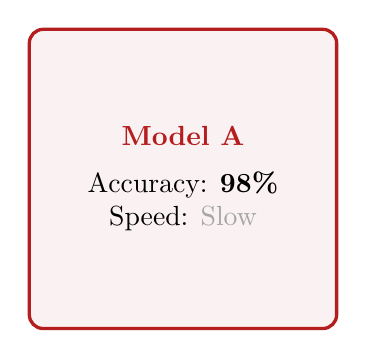
\begin{tikzpicture}
\node[
  draw=AlertRed,
  fill=AlertRed!6,
  rounded corners=5pt,
  line width=1.2pt,
  minimum width=3.6cm,
  minimum height=3.8cm,
  inner sep=10pt
]{
\begin{minipage}{3.2cm}
\centering
{\bfseries\color{AlertRed} Model A}

\vspace{0.5em}

Accuracy: {\bfseries 98\%}

Speed: {\color{gray!70} Slow}
\end{minipage}
};
\end{tikzpicture}

% =====================================================
% MODEL B
% =====================================================
\column{0.33\textwidth}
\centering
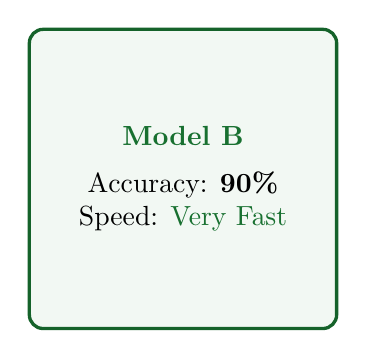
\begin{tikzpicture}
\node[
  draw=GreenOK!70!black,
  fill=GreenOK!6,
  rounded corners=5pt,
  line width=1.2pt,
  minimum width=3.6cm,
  minimum height=3.8cm,
  inner sep=10pt
]{
\begin{minipage}{3.2cm}
\centering
{\bfseries\color{GreenOK!80!black} Model B}

\vspace{0.5em}

Accuracy: {\bfseries 90\%}

Speed: {\color{GreenOK!80!black} Very Fast}
\end{minipage}
};
\end{tikzpicture}

% =====================================================
% MODEL C
% =====================================================
\column{0.33\textwidth}
\centering
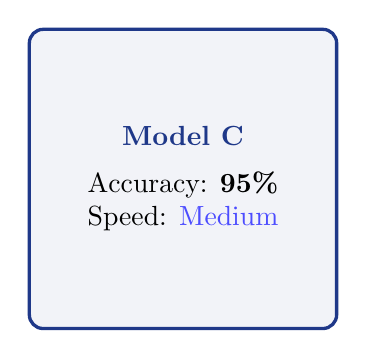
\begin{tikzpicture}
\node[
  draw=NavyBlue,
  fill=NavyBlue!6,
  rounded corners=5pt,
  line width=1.2pt,
  minimum width=3.6cm,
  minimum height=3.8cm,
  inner sep=10pt
]{
\begin{minipage}{3.2cm}
\centering
{\bfseries\color{NavyBlue} Model C}

\vspace{0.5em}

Accuracy: {\bfseries 95\%}

Speed: {\color{blue!70} Medium}
\end{minipage}
};
\end{tikzpicture}

\end{columns}

\vspace{0.8cm}

% =====================================================
% FINAL QUESTION
% =====================================================
\only<2>{
\begin{center}

\begin{tikzpicture}
\node[
  draw=AlertRed,
  fill=AlertRed!5,
  rounded corners=4pt,
  line width=1.2pt,
  inner sep=8pt,
  minimum width=8cm
]{
{\large\bfseries\color{AlertRed}
Which model is optimal?}
};
\end{tikzpicture}
\end{center}
}

\end{frame}

%% =========================================================
%% SLIDE 3 — The Realization (animated)
%% =========================================================
% \begin{frame}[plain]
%   \begin{tikzpicture}[remember picture, overlay]
%     %% Light background wash
%     \fill[NavyBlue!6]
%       (current page.south west) rectangle (current page.north east);
%     %% Top accent bar
%     \fill[NavyBlue]
%       (current page.north west) rectangle
%       ([yshift=-0.45cm]current page.north east);
%     %% Bottom accent bar
%     \fill[NavyBlue]
%       (current page.south west) rectangle
%       ([yshift=0.45cm]current page.south east);
%   \end{tikzpicture}

%   \vspace{1.5em}

%   \begin{center}

%     %% BIG STATEMENT
%     \only<1->{%
%       \begin{tikzpicture}
%         \node[
%           draw=NavyBlue, fill=white,
%           rounded corners=7pt, line width=2pt,
%           inner sep=14pt, minimum width=13cm
%         ] {%
%           \fontsize{22}{28}\selectfont\bfseries\color{NavyBlue}
%           There is no single best model.%
%         };
%       \end{tikzpicture}
%     }

%     \vspace{1.0em}

%     %% REFRAME
%     \only<2->{%
%       \begin{tikzpicture}
%         \node[
%           draw=DarkBlue!40, fill=NavyBlue!10,
%           rounded corners=5pt, line width=1pt,
%           inner sep=10pt, minimum width=11cm
%         ] {%
%           \fontsize{14}{18}\selectfont\color{DarkBlue}
%           It depends on \textbf{what you value.}%
%         };
%       \end{tikzpicture}
%     }

%     \vspace{0.9em}

    % %% INSIGHT LINE
    % \only<3->{%
    %   \begin{tikzpicture}
    %     %% Two opposing labels
    %     \node[
    %       fill=AlertRed, text=white,
    %       rounded corners=4pt, font=\bfseries\normalsize,
    %       inner sep=6pt, minimum width=3.6cm
    %     ] (acc) at (-3.5,0) {Accuracy};

    %     \node[
    %       fill=GreenOK, text=white,
    %       rounded corners=4pt, font=\bfseries\normalsize,
    %       inner sep=6pt, minimum width=3.6cm
    %     ] (spd) at (3.5,0) {Speed};

    %     %% Arrow with label
    %     \draw[-{Stealth[length=7pt]}, AlertRed!70, line width=2pt]
    %       (acc.east) -- ++(1.3,0);
    %     \draw[-{Stealth[length=7pt]}, GreenOK!70, line width=2pt]
    %       (spd.west) -- ++(-1.3,0);

    %     \node[
    %       font=\bfseries\small, text=gray!70!black,
    %       fill=white, draw=gray!40, rounded corners=3pt,
    %       inner sep=4pt
    %     ] at (0,0) {vs};

    %     %% Caption below
    %     \node[
    %       font=\itshape\small, text=gray!60!black,
    %       align=center
    %     ] at (0,-0.75) {Trade-offs are unavoidable.};
    %   \end{tikzpicture}
    % }

%   \end{center}
% \end{frame}

%% =========================================================
%% SLIDE — General Real-World Motivation
%% =========================================================
\begin{frame}{Why Does This Matter? Real-World Trade-Offs}

  \begin{center}
    {\small\itshape Most decisions in the real world force you to balance competing priorities.}
  \end{center}

  \vspace{0.6em}

  \begin{columns}[c]
    \column{0.55\textwidth}

    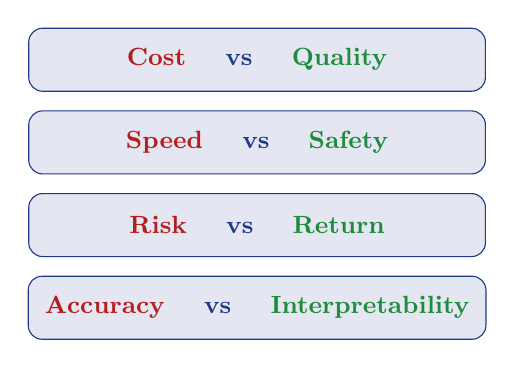
\begin{tikzpicture}[
      bullet/.style={draw=NavyBlue, fill=NavyBlue!12, rounded corners=5pt,
                     minimum width=5.8cm, minimum height=0.80cm,
                     align=center, font=\small\bfseries, text=NavyBlue,
                     inner sep=6pt}
    ]
      \node[bullet] (b1) at (0, 0)    {\textcolor{AlertRed}{Cost} \quad vs \quad \textcolor{GreenOK}{Quality}};
      \node[bullet] (b2) at (0,-1.05) {\textcolor{AlertRed}{Speed} \quad vs \quad \textcolor{GreenOK}{Safety}};
      \node[bullet] (b3) at (0,-2.10) {\textcolor{AlertRed}{Risk} \quad vs \quad \textcolor{GreenOK}{Return}};
      \node[bullet] (b4) at (0,-3.15) {\textcolor{AlertRed}{Accuracy} \quad vs \quad \textcolor{GreenOK}{Interpretability}};
    \end{tikzpicture}

    \column{0.42\textwidth}
    \onslide<2->{
      \begin{block}{}
        \centering
        \textbf{Most real-world problems involve conflicting objectives.}\\[0.4em]
        {\small Improving one goal often means compromising another.}
      \end{block}
    }
  \end{columns}

\end{frame}


%% ---- Two Persons Animated Slide ----

%% Colour palette for cartoon faces
\definecolor{SkinTone}{RGB}{240,195,160}
\definecolor{HairDark}{RGB}{40,30,20}
\definecolor{HairBlue}{RGB}{25,50,110}
\definecolor{ShirtRed}{RGB}{190,40,40}
\definecolor{ShirtTeal}{RGB}{30,120,130}
\definecolor{CloudGreen}{RGB}{50,170,80}
\definecolor{BubbleYellow}{RGB}{240,200,30}

%% Macro: cartoon face
%% Args: cx, cy, scale, hair-style (w=woman / m=man), shirt-color
\newcommand{\cartoonface}[5]{%
  \begin{scope}[shift={(#1,#2)}, scale=#3]
    %% Neck
    \fill[SkinTone] (-0.10,-0.44) rectangle (0.10,-0.20);
    %% Shirt body
    \fill[#5] (-0.55,-1.05) -- (-0.30,-0.44) -- (0.30,-0.44) -- (0.55,-1.05) -- cycle;
    %% Face circle
    \fill[SkinTone, draw=HairDark, line width=0.5pt] (0,0) circle (0.42cm);
    %% Hair
    \ifthenelse{\equal{#4}{w}}{%
      %% Woman: dark bob covering top+sides
      \fill[HairDark]
        (-0.42,0.05) .. controls (-0.48,0.45) and (-0.20,0.72) .. (0,0.72)
        .. controls (0.20,0.72) and (0.48,0.45) .. (0.42,0.05)
        .. controls (0.46,-0.10) and (0.52,-0.25) .. (0.50,-0.38)
        -- (0.38,-0.30)
        .. controls (0.38,0.00) and (0.44,0.05) .. (0.42,0.05)
        -- cycle;
      \fill[HairDark]
        (-0.42,0.05) .. controls (-0.44,0.05) and (-0.38,0.00) .. (-0.38,-0.30)
        -- (-0.50,-0.38)
        .. controls (-0.52,-0.25) and (-0.46,-0.10) .. (-0.42,0.05);
    }{%
      %% Man: short neat hair on top only
      \fill[HairDark]
        (-0.42,0.08) .. controls (-0.44,0.40) and (-0.18,0.68) .. (0,0.68)
        .. controls (0.18,0.68) and (0.44,0.40) .. (0.42,0.08) -- cycle;
    }
    %% Eyes (white + pupil)
    \fill[white] (-0.16,0.05) ellipse (0.10cm and 0.07cm);
    \fill[white] ( 0.16,0.05) ellipse (0.10cm and 0.07cm);
    \fill[HairDark] (-0.14,0.05) circle (0.045cm);
    \fill[HairDark] ( 0.18,0.05) circle (0.045cm);
    %% Eyebrows (slightly furrowed = determined look)
    \draw[HairDark, line width=0.6pt] (-0.26,0.17) .. controls (-0.18,0.21) .. (-0.06,0.17);
    \draw[HairDark, line width=0.6pt] ( 0.06,0.17) .. controls ( 0.18,0.21) .. ( 0.26,0.17);
    %% Nose dot
    \fill[SkinTone!60!HairDark] (0,-0.06) circle (0.03cm);
    %% Mouth (slight smile)
    \draw[HairDark, line width=0.7pt]
      (-0.14,-0.18) .. controls (-0.07,-0.26) and (0.07,-0.26) .. (0.14,-0.18);
    %% Ear marks
    \fill[SkinTone, draw=HairDark, line width=0.4pt]
      (-0.44,-0.03) ellipse (0.07cm and 0.10cm);
    \fill[SkinTone, draw=HairDark, line width=0.4pt]
      ( 0.44,-0.03) ellipse (0.07cm and 0.10cm);
  \end{scope}
}

\begin{frame}{Real-World Example: Buying a Car}

\begin{center}
\begin{tikzpicture}

%% =========================================================
%% PERSON 1  (left, woman)
%% =========================================================
\onslide<1->{

  % Cartoon face
  \cartoonface{-4.2}{0.0}{1.0}{w}{ShirtRed}

  % Name label
  \node[font=\small\bfseries, text=NavyBlue]
    at (-4.2,-1.55) {Person 1};

  % Cloud callout (top right, pointing left)
  \node[
    cloud callout,
    cloud puffs=11,
    cloud puff arc=95,
    minimum width=2.0cm,
    minimum height=1.4cm,
    draw=NavyBlue,
    fill=NavyBlue!15,
    callout absolute pointer={(-3.7,0.2)},
    text width=2.0cm,
    align=center,
    font=\scriptsize\bfseries,
    inner sep=1.8pt,
    line width=1.1pt
  ] at (-0.9,1.8)
  {
    \textcolor{AlertRed}
    {``I want a car with minimum fuel consumption''}
  };
}

%% =========================================================
%% PERSON 2  (right, man)
%% =========================================================
\onslide<2->{

  % Cartoon face
  \cartoonface{4.2}{0.0}{1.0}{m}{ShirtTeal}

  % Name label
  \node[font=\small\bfseries, text=NavyBlue]
    at (4.2,-1.55) {Person 2};

  % Cloud callout (bottom left, pointing right)
  \node[
    cloud callout,
    cloud puffs=11,
    cloud puff arc=95,
    minimum width=2.0cm,
    minimum height=1.4cm,
    draw=CloudGreen,
    fill=CloudGreen!18,
    callout absolute pointer={(3.7,0.2)},
    text width=2.0cm,
    align=center,
    font=\scriptsize\bfseries,
    inner sep=1.8pt,
    line width=1.1pt
  ] at (0.9,-1.1)
  {
    \textcolor{GreenOK}
    {``I want a car with maximum speed limit''}
  };
}

\end{tikzpicture}
\end{center}

\onslide<3->{
\begin{center}
  \alert{\textbf{Both objectives matter --- but they conflict with each other!}}
\end{center}
}

\end{frame}

\begin{frame}{A Real-World Example: Buying a Car}

\begin{center}
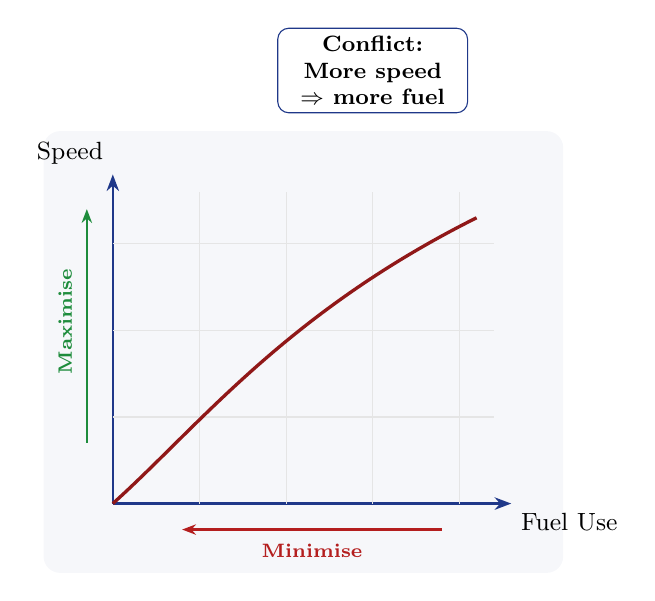
\begin{tikzpicture}[scale=1.1]

  % Soft background panel
  \fill[NavyBlue!4, rounded corners=6pt]
        (-0.8,-0.8) rectangle (5.2,4.3);

  % Axes
  \draw[-{Stealth[length=6pt]}, thick, NavyBlue]
        (0,0) -- (4.6,0);

  \draw[-{Stealth[length=6pt]}, thick, NavyBlue]
        (0,0) -- (0,3.8);

  % Axis labels
  \node[below right, font=\small]
        at (4.6,0) {Fuel Use};

  \node[above left, font=\small]
        at (0,3.8) {Speed};

  % Light grid
  \draw[gray!20, thin]
        (1,0)--(1,3.6)
        (2,0)--(2,3.6)
        (3,0)--(3,3.6)
        (4,0)--(4,3.6);

  \draw[gray!20, thin]
        (0,1)--(4.4,1)
        (0,2)--(4.4,2)
        (0,3)--(4.4,3);

  % RANDOM TRADE-OFF CURVE (smooth Bezier)
  \draw[very thick, AlertRed!80!black]
        (0,0)
        .. controls (1.0,0.9)
        and (2.0,2.2)
        .. (4.2,3.3);

  % OUTSIDE minimise (x-axis direction)
  \node[AlertRed, font=\scriptsize\bfseries]
        at (2.3,-0.55) {Minimise};

  \draw[AlertRed, thick, -{Stealth[length=5pt]}]
        (3.8,-0.30) -- (0.8,-0.30);

  % OUTSIDE maximise (y-axis direction)
  \node[GreenOK, font=\scriptsize\bfseries, rotate=90]
        at (-0.55,2.1) {Maximise};

  \draw[GreenOK, thick, -{Stealth[length=5pt]}]
        (-0.30,0.7) -- (-0.30,3.4);

  % Transparent conflict annotation box
  \node[
    draw=NavyBlue,
    fill=none,
    rounded corners=4pt,
    font=\footnotesize\bfseries,
    align=center,
    inner sep=3pt,
    text width=2.2cm
  ]
  at (3.0,5.0)
  {Conflict:\\ More speed $\Rightarrow$ more fuel};

\end{tikzpicture}
\end{center}

\end{frame}
\begin{frame}{Four Cars on the Shortlist}
  They agree on four candidate cars. Can we shrink the list?

  \vspace{0.4em}
  \begin{columns}[c]
    \column{0.52\textwidth}
    \begin{center}
    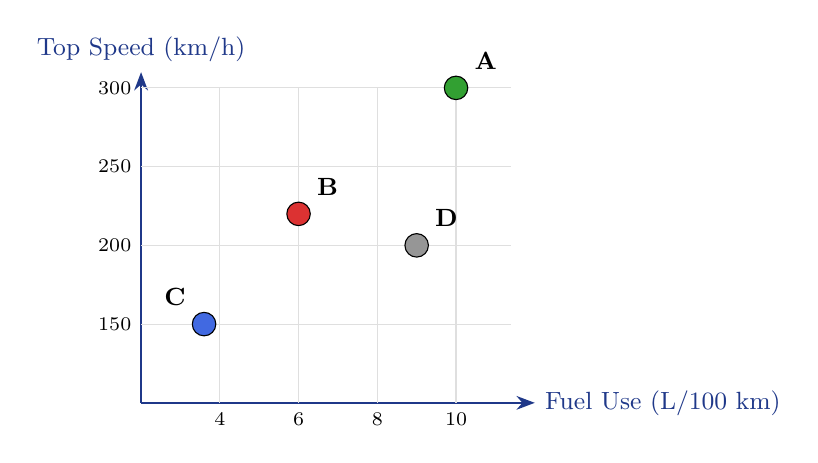
\begin{tikzpicture}[scale=1.0]
      % axes
      \draw[-{Stealth}, thick, NavyBlue] (0,0) -- (5.0,0)
            node[right, font=\small] {Fuel Use (L/100 km)};
      \draw[-{Stealth}, thick, NavyBlue] (0,0) -- (0,4.2)
            node[above, font=\small] {Top Speed (km/h)};

      % grid
      \foreach \x in {1,2,3,4}
        \draw[gray!25,thin] (\x,0)--(\x,4.0);
      \foreach \y in {1,2,3,4}
        \draw[gray!25,thin] (0,\y)--(4.7,\y);

      % axis labels
      \foreach \x/\lbl in {1/4, 2/6, 3/8, 4/10}
        \node[font=\scriptsize, below] at (\x,0) {\lbl};
      \foreach \y/\lbl in {1/150, 2/200, 3/250, 4/300}
        \node[font=\scriptsize, left] at (0,\y) {\lbl};

      % Car A
      \onslide<1->{
        \node[circle, fill=CarGreen, draw=black, inner sep=3pt,
              label={[font=\small\bfseries]above right:A}]
              at (4.0, 4.0) {};
      }

      % Car B
      \onslide<2->{
        \node[circle, fill=CarRed, draw=black, inner sep=3pt,
              label={[font=\small\bfseries]above right:B}]
              at (2.0, 2.4) {};
      }

      % Car C
      \onslide<3->{
        \node[circle, fill=CarBlue, draw=black, inner sep=3pt,
              label={[font=\small\bfseries]above left:C}]
              at (0.8, 1.0) {};
      }

      % Car D
      \onslide<4->{
        \node[circle, fill=CarGray, draw=black, inner sep=3pt,
              label={[font=\small\bfseries]above right:D}]
              at (3.5, 2.0) {};
      }

    \end{tikzpicture}
    \end{center}

    \column{0.45\textwidth}
    \small
    \begin{tabular}{ccc}
      \toprule
      \textbf{Car} & \textbf{Speed} & \textbf{Fuel} \\
      \midrule

      \onslide<1->{\textcolor{CarGreen}{\textbf{A}}} & \onslide<1->{300 km/h} & \onslide<1->{10 L/100} \\

      \onslide<2->{\textcolor{CarRed}{\textbf{B}}}   & \onslide<2->{220 km/h} & \onslide<2->{ 6 L/100} \\

      \onslide<3->{\textcolor{CarBlue}{\textbf{C}}} & \onslide<3->{150 km/h} & \onslide<3->{ 4 L/100} \\

      \onslide<4->{\textcolor{CarGray}{\textbf{D}}}  & \onslide<4->{200 km/h} & \onslide<4->{ 9 L/100} \\

      \bottomrule
    \end{tabular}

    \vspace{0.8em}
    \onslide<5->{
      \textbf{Goal:} Maximise speed,\\
      \phantom{\textbf{Goal:}} Minimise fuel use.

      \vspace{0.4em}
      \alert{Can we remove any car?}
    }

  \end{columns}
\end{frame}

% %% ============================================================
% %% SECTION 2
% %% ============================================================
\begin{frame}[plain]
  \begin{center}
    \vspace{3em}
    {\Huge\bfseries\color{NavyBlue} Dominance \& Non-Domination}
  \end{center}
\end{frame}

%% =========================================================
%% DOMINANCE — Merged Slide: Intuition + Formal Conditions
%% =========================================================
\begin{frame}{The Key Concept: Dominance}

\begin{center}

\onslide<1->{
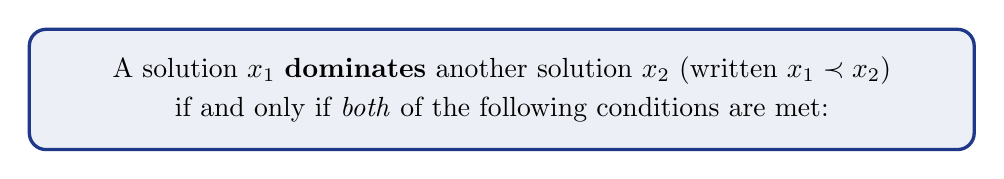
\begin{tikzpicture}
  \node[draw=NavyBlue, fill=NavyBlue!8, rounded corners=6pt,
        line width=1.2pt, inner sep=10pt, minimum width=12cm, align=center]
  {%
    A solution $x_1$ \textbf{dominates} another solution $x_2$
    (written $x_1 \prec x_2$)\\[0.2em]
    if and only if \emph{both} of the following conditions are met:
  };
\end{tikzpicture}
}

\vspace{0.8em}

\onslide<2->{

\begin{tikzpicture}
  \node[draw=NavyBlue, fill=NavyBlue!10, rounded corners=5pt,
        line width=1pt, inner sep=10pt, minimum width=12cm, align=left, font=\normalsize]
  {%
    \textbf{\textcolor{NavyBlue}{Condition\ 1 --- No Worse in All Objectives:}}\\[0.3em]
    $x_1$ is \textbf{no worse} than $x_2$ in \emph{every} objective.
  };
\end{tikzpicture}
}

\vspace{0.6em}

\onslide<3->{
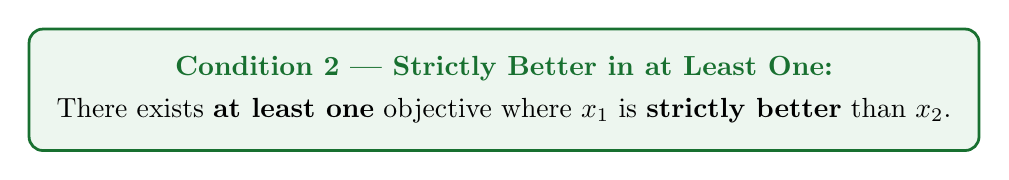
\begin{tikzpicture}
  \node[draw=GreenOK!80!black, fill=GreenOK!8, rounded corners=5pt,
        line width=1pt, inner sep=10pt, minimum width=12cm, align=center, font=\normalsize]
  {%
    \textbf{\textcolor{GreenOK!80!black}{Condition\ 2 --- Strictly Better in at Least One:}}\\[0.3em]
    There exists \textbf{at least one} objective where $x_1$ is \textbf{strictly better} than $x_2$.
  };
\end{tikzpicture}
}

\end{center}

\end{frame}


%% =========================================================
%% DOMINANCE — Slide D: Visual — All Cars on Plot (animated)
%% =========================================================
\begin{frame}{Visualising Dominance: All Four Cars}

  \begin{columns}[c]
    \column{0.55\textwidth}
    \begin{center}
    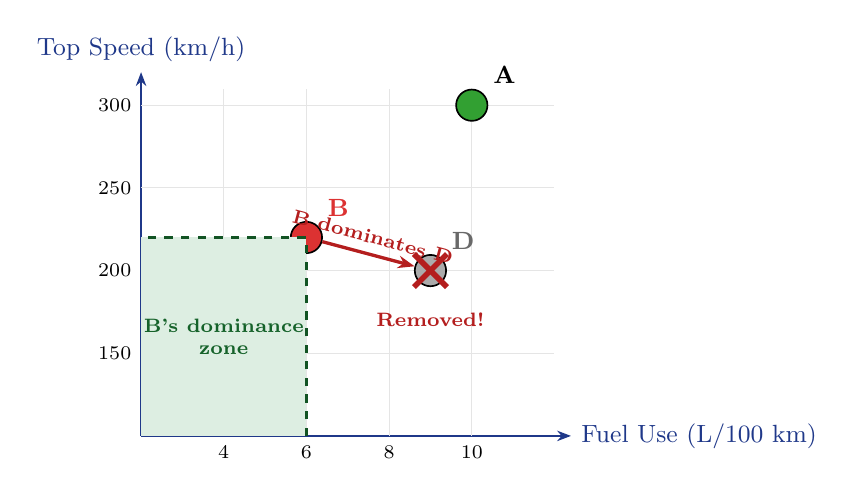
\begin{tikzpicture}[scale=1.05]
      % Axes
      \draw[-{Stealth[length=5pt]}, NavyBlue, thick]
        (0,0) -- (5.2,0) node[right, font=\small] {Fuel Use (L/100 km)};
      \draw[-{Stealth[length=5pt]}, NavyBlue, thick]
        (0,0) -- (0,4.4) node[above, font=\small] {Top Speed (km/h)};
      % Grid
      \foreach \x in {1,2,3,4}
        \draw[gray!20,thin] (\x,0)--(\x,4.2);
      \foreach \y in {1,2,3,4}
        \draw[gray!20,thin] (0,\y)--(5.0,\y);
      % Tick labels
      \foreach \x/\lbl in {1/4, 2/6, 3/8, 4/10}
        \node[font=\scriptsize, below] at (\x,0) {\lbl};
      \foreach \y/\lbl in {1/150, 2/200, 3/250, 4/300}
        \node[font=\scriptsize, left] at (0,\y) {\lbl};

      % Step 1: Show all four cars
      \onslide<1->{
        \node[circle, fill=CarGreen, draw=black, line width=0.6pt, inner sep=4pt,
              label={[font=\small\bfseries]above right:A}] (A) at (4.0,4.0) {};
        \node[circle, fill=CarRed, draw=black, line width=0.6pt, inner sep=4pt,
              label={[font=\small\bfseries, text=CarRed]above right:B}] (B) at (2.0,2.4) {};
        \node[circle, fill=CarGreen, draw=black, line width=0.6pt, inner sep=4pt,
              label={[font=\small\bfseries]above left:C}] (C) at (0.8,1.0) {};
        \node[circle, fill=CarGray!80, draw=black, line width=0.6pt, inner sep=4pt,
              label={[font=\small\bfseries, text=CarGray!70!black]above right:D}] (D) at (3.5,2.0) {};
      }

      % Step 2: Highlight B's dominance zone
      \onslide<2->{
        \fill[GreenOK!15] (0,0) rectangle (2.0,2.4);
        \draw[dashed, GreenOK!60!black, thick]
          (2.0,0) -- (2.0,2.4) -- (0,2.4);
        \node[font=\scriptsize\bfseries, text=GreenOK!70!black, align=center]
          at (1.0,1.2) {B's dominance\\zone};
      }

      % Step 3: Arrow from B to D
      \onslide<3->{
        \draw[-{Stealth[length=6pt]}, AlertRed, very thick]
          (B) -- (D) node[midway, above,  font=\scriptsize\bfseries, text=AlertRed, sloped]
          {B dominates D};
      }

      % Step 4: Cross out D
      \onslide<4->{
        \draw[AlertRed, very thick, line width=2pt] (3.3,1.8) -- (3.7,2.2);
        \draw[AlertRed, very thick, line width=2pt] (3.7,1.8) -- (3.3,2.2);
        \node[font=\scriptsize\bfseries, text=AlertRed] at (3.5,1.4) {Removed!};
      }

    \end{tikzpicture}
    \end{center}

    \column{0.42\textwidth}

    \onslide<1->{
      \textbf{Our four candidates:}\\[0.3em]
      \small
      \begin{tabular}{lcc}
        \toprule
        \textbf{Car} & \textbf{Speed} & \textbf{Fuel} \\
        \midrule
        A & 300 km/h & 10 L \\
        B & 220 km/h & 6 L \\
        C & 150 km/h & 4 L \\
        D & 200 km/h & 9 L \\
        \bottomrule
      \end{tabular}
    }

    \vspace{0.6em}

    \onslide<2->{
      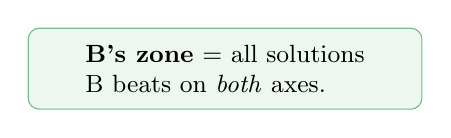
\begin{tikzpicture}
        \node[draw=GreenOK!60, fill=GreenOK!8, rounded corners=4pt,
              inner sep=6pt, minimum width=5.0cm, align=left, font=\small] {%
          \textbf{B's zone} = all solutions\\
          B beats on \emph{both} axes.
        };
      \end{tikzpicture}
    }

    \vspace{0.4em}

    \onslide<3->{
      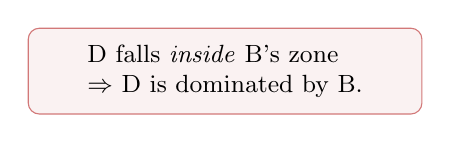
\begin{tikzpicture}
        \node[draw=AlertRed!60, fill=AlertRed!6, rounded corners=4pt,
              inner sep=6pt, minimum width=5.0cm, align=left, font=\small] {%
          D falls \emph{inside} B's zone\\
          $\Rightarrow$ D is dominated by B.
        };
      \end{tikzpicture}
    }

    \vspace{0.4em}

    \onslide<4->{
      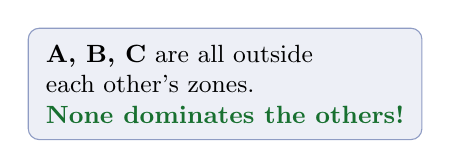
\begin{tikzpicture}
        \node[draw=NavyBlue!50, fill=NavyBlue!8, rounded corners=4pt,
              inner sep=6pt, minimum width=5.0cm, align=left, font=\small] {%
          \textbf{A, B, C} are all outside\\
          each other's zones.\\
          \textcolor{GreenOK!80!black}{\bfseries None dominates the others!}
        };
      \end{tikzpicture}
    }

  \end{columns}
\end{frame}

%% =========================================================
%% MERGED — Pairwise Comparisons + Pareto Front
%% =========================================================
\begin{frame}{The Remaining Cars Form the Pareto Front}

\begin{columns}[c]

% ================= LEFT: Compact pairwise summary =================
\column{0.48\textwidth}

\onslide<1->{
\begin{center}
{\small\itshape Can A, B, or C dominate each other?}
\end{center}

\vspace{0.3em}

\small
\begin{tabular}{cccc}
  \toprule
  \textbf{Pair} & \textbf{Speed} & \textbf{Fuel} & \textbf{Result} \\
  \midrule
  A vs B & A \textcolor{GreenOK}{\checkmark} & B \textcolor{GreenOK}{\checkmark} & \textbf{No dominance} \\
  A vs C & A \textcolor{GreenOK}{\checkmark} & C \textcolor{GreenOK}{\checkmark} & \textbf{No dominance} \\
  B vs C & B \textcolor{GreenOK}{\checkmark} & C \textcolor{GreenOK}{\checkmark} & \textbf{No dominance} \\
  \bottomrule
\end{tabular}
}

\vspace{0.5em}

\onslide<2->{
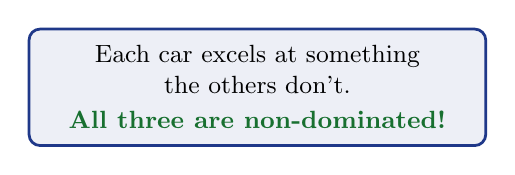
\begin{tikzpicture}
  \node[draw=NavyBlue, fill=NavyBlue!8, rounded corners=4pt,
        line width=1pt, inner sep=6pt, minimum width=5.8cm,
        align=center, font=\small]
  {%
    Each car excels at something\\
    the others don't.\\[0.2em]
    \textcolor{GreenOK!80!black}{\bfseries All three are non-dominated!}
  };
\end{tikzpicture}
}


% ================= RIGHT: Pareto front graph =================
\column{0.50\textwidth}

\onslide<2->{
\begin{center}
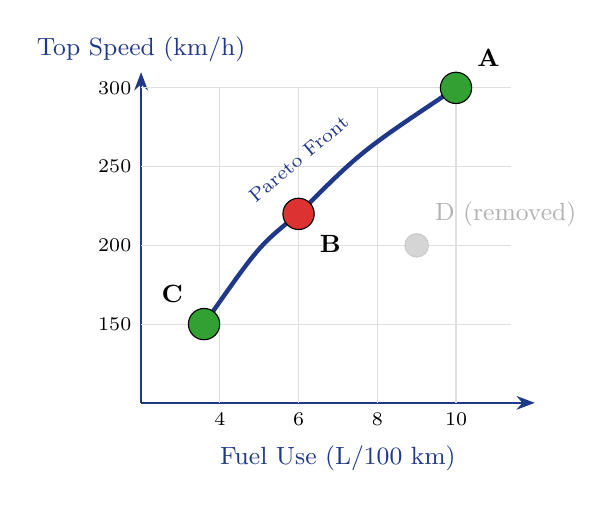
\begin{tikzpicture}[scale=1.0]
  \draw[-{Stealth}, thick, NavyBlue] (0,0) -- (5.0,0)
        node[font=\small] at (2.5,-0.7) {Fuel Use (L/100 km)};
  \draw[-{Stealth}, thick, NavyBlue] (0,0) -- (0,4.2)
        node[above, font=\small] {Top Speed (km/h)};
  \foreach \x in {1,2,3,4}
    \draw[gray!25,thin] (\x,0)--(\x,4.0);
  \foreach \y in {1,2,3,4}
    \draw[gray!25,thin] (0,\y)--(4.7,\y);
  \foreach \x/\lbl in {1/4, 2/6, 3/8, 4/10}
    \node[font=\scriptsize, below] at (\x,0) {\lbl};
  \foreach \y/\lbl in {1/150, 2/200, 3/250, 4/300}
    \node[font=\scriptsize, left] at (0,\y) {\lbl};
  % Non-dominated front curve
  \draw[NavyBlue, ultra thick] (0.8,1.0) .. controls (1.5,2.0) .. (2.0,2.4)
                                         .. controls (2.8,3.2) .. (4.0,4.0);
  \node[font=\scriptsize, text=NavyBlue, rotate=40] at (2,3.1)
        {Pareto Front};
  % Cars A, B, C (non-dominated)
  \node[circle, fill=CarGreen, draw=black, inner sep=4pt,
        label={[font=\small\bfseries]above right:A}] (A) at (4.0, 4.0) {};
  \node[circle, fill=CarRed,   draw=black, inner sep=4pt,
        label={[font=\small\bfseries]below right:B}] (B) at (2.0, 2.4) {};
  \node[circle, fill=CarGreen, draw=black, inner sep=4pt,
        label={[font=\small\bfseries]above left:C}]  (C) at (0.8, 1.0) {};
  % D faded
  \node[circle, fill=CarGray!40, draw=gray!40, inner sep=3pt,
        label={[font=\small, text=gray!60]above right:D (removed)}]
        (D) at (3.5, 2.0) {};
\end{tikzpicture}
\end{center}
}

\end{columns}
\end{frame}

\begin{frame}{The Goal of Multi-Objective Optimization}

% ------------------------------------------------
% Fundamental Goal (Top)
% ------------------------------------------------
\begin{block}{The Fundamental Goal}
Multi-objective optimization aims to 
\textbf{find (or approximate) the entire non-dominated set} — 
giving the decision-maker the full picture of trade-offs.
\end{block}

\vspace{0.6em}

% ------------------------------------------------
% Concept Diagram (Middle)
% ------------------------------------------------
\begin{center}
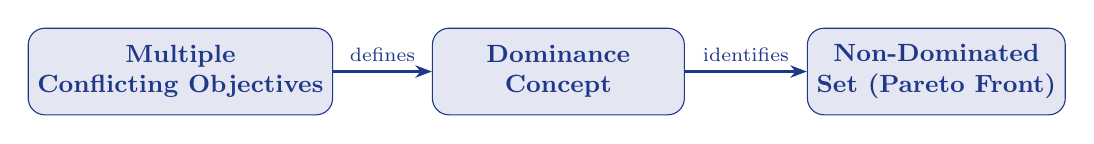
\begin{tikzpicture}[
  box/.style={
    draw=NavyBlue,
    fill=NavyBlue!12,
    rounded corners=6pt,
    minimum width=3.2cm,
    minimum height=1.1cm,
    align=center,
    font=\small\bfseries,
    text=NavyBlue
  },
  arrow/.style={-{Stealth[length=6pt]}, NavyBlue, thick}
]

\node[box] (A) at (0,0)
  {Multiple\\ Conflicting Objectives};

\node[box] (B) at (4.8,0)
  {Dominance\\ Concept};

\node[box] (C) at (9.6,0)
  {Non-Dominated\\ Set (Pareto Front)};

\draw[arrow] (A) -- (B)
  node[midway, above, font=\scriptsize]{defines};

\draw[arrow] (B) -- (C)
  node[midway, above, font=\scriptsize]{identifies};

\end{tikzpicture}
\end{center}

\vspace{0.8em}

% ------------------------------------------------
% Final Distilled Statement (Bottom)
% ------------------------------------------------
% \begin{center}
% \begin{tikzpicture}
% \node[
%   draw=GreenOK!80!black,
%   fill=GreenOK!12,
%   rounded corners=6pt,
%   line width=1.2pt,
%   inner sep=8pt,
%   text width=9.5cm,
%   text centered,
%   font=\small
% ]
% {
% \textbf{Discover all trade-off solutions that cannot be improved without sacrifice.}
% };
% \end{tikzpicture}
% \end{center}

\end{frame}
%% ============================================================
%% EVOLUTIONARY ALGORITHM SLIDES — BEGINNER FRIENDLY VERSION
%% Insert these slides AFTER the Summary frame, BEFORE \end{document}
%% ============================================================


%% ============================================================
%% SECTION DIVIDER
%% ============================================================
\begin{frame}{What if there are millions of solutions?}

  % STEP 1 — Show only the question
  \onslide<1->{
  \begin{block}{The Challenge}
    Imagine you have \textbf{millions of possible solutions} to a problem.
    You cannot try them all. How do you find a good one \emph{fast}?
  \end{block}
  }

  \vspace{0.1em}

  \begin{columns}[T]

    % STEP 2 — Random search appears
    \column{0.48\textwidth}
    \onslide<2->{
    \textbf{A bad strategy: Random Search}\\[0.4em]
    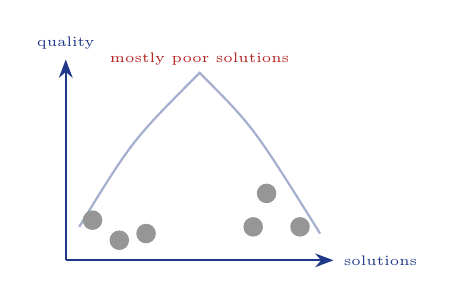
\begin{tikzpicture}[scale=0.85]
      \draw[-{Stealth}, NavyBlue, thick] (0,0)--(4,0)
            node[right, font=\tiny]{solutions};
      \draw[-{Stealth}, NavyBlue, thick] (0,0)--(0,3)
            node[above, font=\tiny]{quality};

      \draw[NavyBlue!40, thick]
            (0.2,0.5) .. controls (1,1.8) .. (2.0,2.8)
            .. controls (2.8,2.0) .. (3.8,0.4);

      \foreach \x/\y in {0.4/0.6, 1.2/0.4, 3.5/0.5, 0.8/0.3, 3.0/1.0, 2.8/0.5}
        \node[circle, fill=CarGray, inner sep=2.5pt] at (\x,\y) {};

      \node[font=\tiny, text=AlertRed] at (2.0, 3.0) {mostly poor solutions};
    \end{tikzpicture}

    {\small Picking random solutions wastes most attempts on bad regions.}
    }

    % STEP 3 — Guided improvement appears
    \column{0.48\textwidth}
    \onslide<3->{
    \textbf{A smarter strategy: Learn \& Improve}\\[0.4em]
    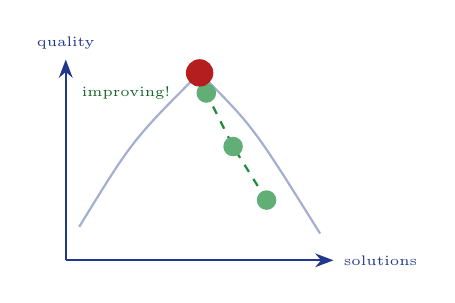
\begin{tikzpicture}[scale=0.85]
      \draw[-{Stealth}, NavyBlue, thick] (0,0)--(4,0)
            node[right, font=\tiny]{solutions};
      \draw[-{Stealth}, NavyBlue, thick] (0,0)--(0,3)
            node[above, font=\tiny]{quality};

      \draw[NavyBlue!40, thick]
            (0.2,0.5) .. controls (1,1.8) .. (2.0,2.8)
            .. controls (2.8,2.0) .. (3.8,0.4);

      \draw[-{Stealth}, GreenOK, thick, dashed]
            (3.0,0.9) -- (2.5,1.7) -- (2.1,2.5) -- (2.0,2.8);

      \foreach \x/\y in {3.0/0.9, 2.5/1.7, 2.1/2.5}
        \node[circle, fill=GreenOK!70, inner sep=2.5pt] at (\x,\y) {};

      \node[circle, fill=AlertRed, inner sep=3.5pt] at (2.0,2.8) {};
      \node[font=\tiny, text=GreenOK!70!black] at (0.9,2.5) {improving!};
    \end{tikzpicture}

    {\small Use what you've learned so far to guide the next attempt.}
    }

  \end{columns}

  % STEP 4 — Final conclusion line appears last
  \vspace{0.1em}
  \onslide<4->{
  \begin{center}
    \textbf{Evolutionary Algorithms do exactly this — guided, improving search.}
  \end{center}
  }

\end{frame}


%% ============================================================
%% SLIDE 2 — The Nature Analogy (plain, no jargon)
%% ============================================================
% \begin{frame}{The Big Idea: Borrow from Nature}

%   \begin{center}
%   \begin{tikzpicture}[
%     box/.style={draw=NavyBlue, fill=NavyBlue!10, rounded corners=8pt,
%                 minimum width=3.2cm, minimum height=1.4cm,
%                 align=center, font=\small\bfseries, text=NavyBlue,
%                 inner sep=6pt},
%     nat/.style={draw=GreenOK!80!black, fill=GreenOK!10, rounded corners=8pt,
%                 minimum width=3.2cm, minimum height=1.4cm,
%                 align=center, font=\small\bfseries, text=GreenOK!60!black,
%                 inner sep=6pt},
%     arr/.style={-{Stealth[length=6pt]}, NavyBlue, thick}
%   ]

%     \node[font=\bfseries, NavyBlue] at (-3.5, 2.4) {In Nature:};
%     \node[font=\bfseries, NavyBlue] at ( 3.5, 2.4) {In Our Algorithm:};

%     % Nature column
%     \node[nat] (n1) at (-3.5,  1.2) {Animals in\\a population};
%     \node[nat] (n2) at (-3.5, -0.2) {Stronger ones\\survive \& reproduce};
%     \node[nat] (n3) at (-3.5, -1.6) {Offspring inherit\\traits (with changes)};
%     \node[nat] (n4) at (-3.5, -3.0) {Population gets\\better over time};

%     \draw[arr] (n1)--(n2); \draw[arr] (n2)--(n3); \draw[arr] (n3)--(n4);

%     % Algorithm column
%     \node[box] (a1) at (3.5,  1.2) {Candidate\\solutions};
%     \node[box] (a2) at (3.5, -0.2) {Better solutions\\chosen as parents};
%     \node[box] (a3) at (3.5, -1.6) {New solutions created\\by mixing parents};
%     \node[box] (a4) at (3.5, -3.0) {Solutions improve\\generation by generation};

%     \draw[arr] (a1)--(a2); \draw[arr] (a2)--(a3); \draw[arr] (a3)--(a4);

%     % Horizontal mapping arrows
%     \foreach \y in {1.2, -0.2, -1.6, -3.0}
%       \draw[{Stealth[length=5pt]}-{Stealth[length=5pt]}, AlertRed!70, thick,
%             dashed] (-1.8,\y) -- (1.8,\y);

%     % divider
%     \draw[NavyBlue!30, thick] (0, 2.0) -- (0,-3.6);
%   \end{tikzpicture}
%   \end{center}
% \end{frame}




%% ============================================================
%% SLIDE 4 — The 3 Steps, one at a time (animated reveal)
%% ============================================================
\begin{frame}{Three Steps — The Evolutionary Cycle}

\begin{center}
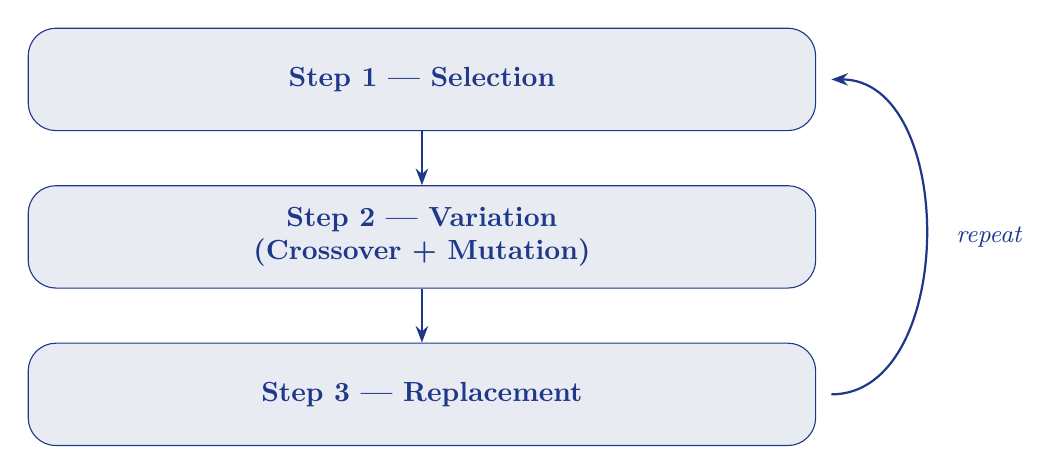
\begin{tikzpicture}[
  pill/.style={
    draw=NavyBlue,
    fill=NavyBlue!10,
    rounded corners=10pt,
    minimum width=10cm,
    minimum height=1.3cm,
    align=center,
    font=\bfseries,
    text=NavyBlue
  },
  sub/.style={
    font=\small,
    text width=9cm,
    align=center
  }
]

% ---------------- STEP 1 ----------------
\onslide<1->{
\node[pill] (s1) at (0,3.0)
{Step 1 — Selection};

% \node[sub] at (0,2.3)
% {Choose promising parents based on objective values.};
}

% ---------------- STEP 2 ----------------
\onslide<2->{
\node[pill] (s2) at (0,1.0)
{Step 2 — Variation \\ (Crossover + Mutation)};

% \node[sub] at (0,0.3)
% {Crossover + Mutation \\
% Generate new candidate solutions.};

\draw[-{Stealth[length=6pt]}, thick, NavyBlue]
(s1.south) -- (s2.north);
}

% ---------------- STEP 3 ----------------
\onslide<3->{
\node[pill] (s3) at (0,-1.0)
{Step 3 — Replacement};

% \node[sub] at (0,-1.7)
% {Insert better offspring. Keep population size fixed.};

\draw[-{Stealth[length=6pt]}, thick, NavyBlue]
(s2.south) -- (s3.north);
}

% ---------------- REPEAT LOOP ----------------
\onslide<4->{
\draw[-{Stealth[length=6pt]}, thick, NavyBlue]
(5.2,-1.0) .. controls +(1.6,0) and +(1.6,0) .. (5.2,3.0);

\node[font=\small\itshape, text=NavyBlue]
at (7.2,1.0) {repeat};
}

\end{tikzpicture}
\end{center}

\end{frame}


%% ============================================================
%% SLIDE 5 — Selection explained with analogy
%% ============================================================
\begin{frame}{Step 1 in Detail: Selection}

  \begin{columns}[T]
    \column{0.50\textwidth}

    \begin{block}{What is Selection?}
      We look at every solution in the population and give
      \textbf{better-scoring solutions a higher chance} of being chosen
      as parents. Worse solutions can still be chosen — just less often.
    \end{block}


    \vspace{0.1em}
    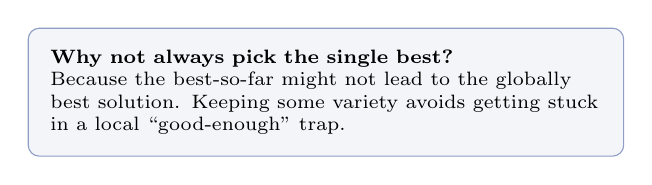
\begin{tikzpicture}
      \node[draw=NavyBlue!50, fill=NavyBlue!5, rounded corners=4pt,
            font=\scriptsize, inner sep=8pt, text width=7cm]
        {\textbf{Why not always pick the single best?}\\
         Because the best-so-far might not lead to the
         globally best solution. Keeping some variety avoids getting
         stuck in a local ``good-enough'' trap.};
    \end{tikzpicture}

    \column{0.47\textwidth}
    \begin{center}
    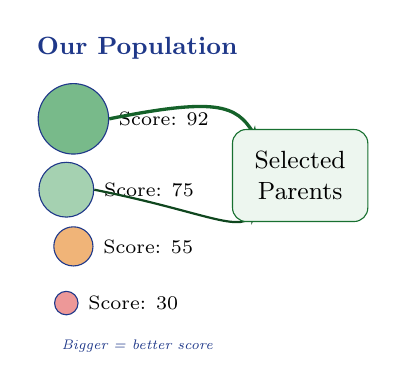
\begin{tikzpicture}[scale=0.9]
      % Population of 6 solutions as circles, sized by fitness
      \node[font=\small\bfseries, NavyBlue] at (1.5, 3.8) {Our Population};

      % solution nodes — size hints quality
      \node[circle, draw=NavyBlue, fill=GreenOK!60, inner sep=9pt,
            label={[font=\scriptsize]right:Score: 92}]   (A) at (0.6, 2.8) {};
      \node[circle, draw=NavyBlue, fill=GreenOK!40, inner sep=7pt,
            label={[font=\scriptsize]right:Score: 75}]   (B) at (0.5, 1.8) {};
      \node[circle, draw=NavyBlue, fill=CarOrange!60, inner sep=5pt,
            label={[font=\scriptsize]right:Score: 55}]   (C) at (0.6, 1.0) {};
      \node[circle, draw=NavyBlue, fill=CarRed!50, inner sep=3pt,
            label={[font=\scriptsize]right:Score: 30}]   (D) at (0.5, 0.2) {};

      % selection arrows from top two
      \draw[-{Stealth[length=5pt]}, GreenOK!70!black, very thick]
            (A.east) .. controls +(1.5,0.3) and +(-0.3,0.5) .. (3.2, 2.5);
      \draw[-{Stealth[length=5pt]}, GreenOK!50!black, thick]
            (B.east) .. controls +(1.5,-0.3) and +(-0.3,-0.3) .. (3.2, 1.5);

      % "selected parents" box
      \node[draw=GreenOK!80!black, fill=GreenOK!8, rounded corners=5pt,
            font=\small, inner sep=8pt, align=center] at (3.8, 2.0)
            {Selected\\Parents};

      \node[font=\tiny\itshape, text=NavyBlue] at (1.5, -0.4)
            {Bigger = better score};
    \end{tikzpicture}
    \end{center}
  \end{columns}
\end{frame}


%% ============================================================
%% SLIDE 6 — Crossover explained with analogy
%% ============================================================
\begin{frame}{Step 2a: Crossover — Mixing Parents}

  \begin{block}{What is Crossover?}
    Take \textbf{two parent solutions} and combine parts of each to
    create a \textbf{child solution}. The child gets some traits from
    Parent A and some from Parent B.
  \end{block}

  \vspace{0.4em}

  \begin{center}
  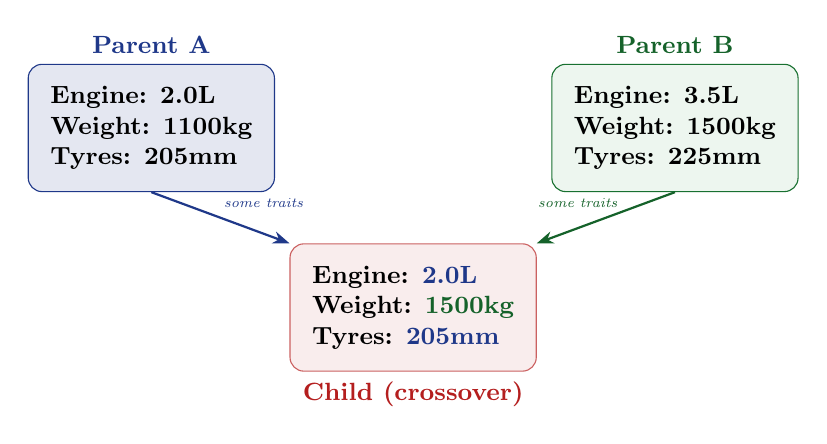
\begin{tikzpicture}[scale=0.95]

    % Parent A
    \node[draw=NavyBlue, fill=NavyBlue!12, rounded corners=5pt,
          font=\small\bfseries, inner sep=8pt, align=left,
          label={[font=\small\bfseries, NavyBlue]above:Parent A}]
          (PA) at (-3.5, 0)
          {Engine: 2.0L\\Weight: 1100kg\\Tyres: 205mm};

    % Parent B
    \node[draw=GreenOK!80!black, fill=GreenOK!8, rounded corners=5pt,
          font=\small\bfseries, inner sep=8pt, align=left,
          label={[font=\small\bfseries, GreenOK!70!black]above:Parent B}]
          (PB) at (3.5, 0)
          {Engine: 3.5L\\Weight: 1500kg\\Tyres: 225mm};

    % Child
    \node[draw=AlertRed!70, fill=AlertRed!8, rounded corners=5pt,
          font=\small\bfseries, inner sep=8pt, align=left,
          label={[font=\small\bfseries, AlertRed]below:Child (crossover)}]
          (CH) at (0, -2.4)
          {Engine: \textcolor{NavyBlue}{2.0L}\\
           Weight: \textcolor{GreenOK!70!black}{1500kg}\\
           Tyres: \textcolor{NavyBlue}{205mm}};

    % Arrows
    \draw[-{Stealth[length=6pt]}, NavyBlue, thick] (PA.south) -- (CH.north west);
    \draw[-{Stealth[length=6pt]}, GreenOK!70!black, thick] (PB.south) -- (CH.north east);

    % Labels on arrows
    \node[font=\tiny\itshape, NavyBlue] at (-2.0,-1.0) {some traits};
    \node[font=\tiny\itshape, GreenOK!70!black] at (2.2,-1.0) {some traits};
  \end{tikzpicture}
  \end{center}

  \vspace{0.2em}
  \begin{center}
    {\small\itshape The child might combine the best aspects of both parents —
    or produce something new entirely!}
  \end{center}
\end{frame}


%% ============================================================
%% SLIDE 7 — Mutation explained
%% ============================================================
\begin{frame}{Step 2b: Mutation — Adding a Little Randomness}

  \begin{columns}[T]
    \column{0.50\textwidth}

    \begin{block}{What is Mutation?}
      After crossover, we \textbf{randomly change} one or a few values
      in the child solution by a small amount.
    \end{block}

    \vspace{0.4em}
    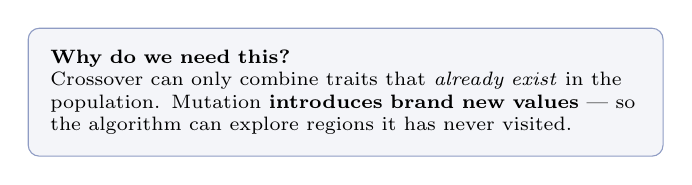
\begin{tikzpicture}
      \node[draw=NavyBlue!50, fill=NavyBlue!5, rounded corners=4pt,
            font=\scriptsize, inner sep=8pt, text width=7.5cm]
        {\textbf{Why do we need this?}\\
    Crossover can only combine traits that \emph{already exist} in the
    population. Mutation \textbf{introduces brand new values} — so the
    algorithm can explore regions it has never visited.};
    \end{tikzpicture}

    \column{0.47\textwidth}
    \begin{center}
    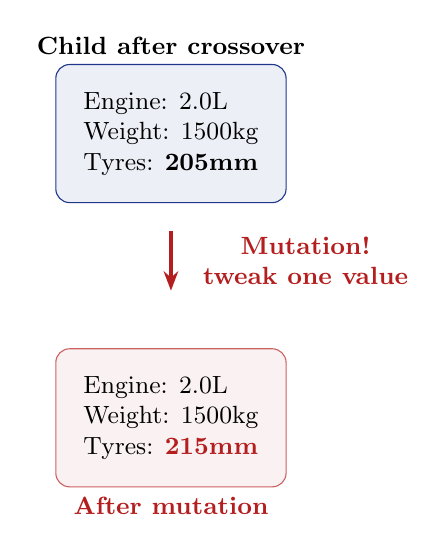
\begin{tikzpicture}[scale=0.95]
      % Before mutation box
      \node[draw=NavyBlue, fill=NavyBlue!8, rounded corners=5pt,
            font=\small, inner sep=10pt, align=left,
            label={[font=\small\bfseries]above:Child after crossover}]
            (bef) at (0, 1.8)
            {Engine: 2.0L\\Weight: 1500kg\\Tyres: \textbf{205mm}};

      % mutation arrow
      \draw[-{Stealth[length=7pt]}, AlertRed, very thick] (0,0.5) -- (0,-0.3);
      \node[font=\small\bfseries, AlertRed, align=center] at (1.8, 0.1)
            {Mutation!\\tweak one value};

      % After mutation box
      \node[draw=AlertRed!70, fill=AlertRed!6, rounded corners=5pt,
            font=\small, inner sep=10pt, align=left,
            label={[font=\small\bfseries, AlertRed]below:After mutation}]
            (aft) at (0,-2.0)
            {Engine: 2.0L\\Weight: 1500kg\\Tyres: \textbf{\textcolor{AlertRed}{215mm}}};

    \end{tikzpicture}
    \end{center}
  \end{columns}
\end{frame}


%% ============================================================
%% SLIDE 9 — Animated Simulation (population cloud moving)
%% ============================================================
\begin{frame}{Let's Watch It Happen: A Visual Simulation}

  \begin{columns}[c]
    \column{0.62\textwidth}
    \begin{center}
    \begin{tikzpicture}[scale=0.88]

      % Axes
      \draw[-{Stealth}, thick, NavyBlue] (0,0)--(5.6,0);
      \draw[-{Stealth}, thick, NavyBlue] (0,0)--(0,4.6);
      \node[font=\small, NavyBlue] at (2.8,-0.4) {Fuel Use (less is better $\leftarrow$)};
      \node[font=\small, NavyBlue, rotate=90] at (-0.55, 2.3) {Speed (more is better $\uparrow$)};

      % Ideal corner shading
      \fill[GreenOK!12] (0,3.0) rectangle (1.8,4.4);
      \node[font=\tiny, text=GreenOK!70!black] at (1.0, 4.3) {ideal region};

      %% === Gen 0: random scattered cloud ===
      \only<1>{
        \node[font=\small\bfseries, NavyBlue] at (3.0, 5.5)
              {Generation 0 — random start};
        \foreach \x/\y in {4.1/0.8, 4.6/1.2, 3.8/0.5, 5.0/1.0, 4.3/1.8,
                            3.5/0.9, 4.7/0.6, 3.2/1.5, 4.9/1.4, 3.0/0.7}
          \node[circle, fill=CarGray!80, draw=gray!60, inner sep=3pt] at (\x,\y) {};
        \node[font=\scriptsize\itshape, text=gray] at (4.0, 5.1)
              {All solutions are poor — scattered with high fuel use, low speed};
      }

      %% === Gen 1: shift begins ===
      \only<2>{
        \node[font=\small\bfseries, NavyBlue] at (3.0, 5.5)
              {Generation 1 — first improvement};
        % old (faded)
        \foreach \x/\y in {4.1/0.8, 4.6/1.2, 3.8/0.5, 5.0/1.0, 4.3/1.8}
          \node[circle, fill=CarGray!25, draw=gray!20, inner sep=3pt] at (\x,\y) {};
        % new (blue)
        \foreach \x/\y in {3.4/1.4, 3.0/1.8, 3.6/2.2, 2.8/1.2, 3.2/2.6,
                            2.5/1.6, 3.8/2.0, 2.2/2.2, 3.0/2.8, 2.6/2.0}
          \node[circle, fill=CarBlue!80, draw=NavyBlue!60, inner sep=3pt] at (\x,\y) {};
        \node[font=\scriptsize\itshape, text=NavyBlue] at (3.5, -1.0)
              {Selection + crossover pulled the cloud toward better regions};
      }

      %% === Gen 2: approaching front ===
      \only<3>{
        \node[font=\small\bfseries, NavyBlue] at (3.0, 5.5)
              {Generation 2 — converging fast};
        % faded gen1
        \foreach \x/\y in {3.4/1.4, 3.0/1.8, 3.6/2.2, 2.8/1.2}
          \node[circle, fill=CarGray!25, draw=gray!20, inner sep=3pt] at (\x,\y) {};
        % new (green)
        \foreach \x/\y in {1.8/2.6, 1.4/3.0, 2.2/3.2, 1.0/3.5,
                            1.6/3.4, 0.8/3.7, 2.0/3.0, 1.2/3.2, 1.9/2.8, 0.6/3.8}
          \node[circle, fill=GreenOK!75, draw=GreenOK!60!black, inner sep=3pt]
                at (\x,\y) {};
        % dashed emerging front
        \draw[AlertRed, dashed, thick]
              (0.4,3.9) .. controls (1.0,3.4) .. (2.0,2.8)
              .. controls (2.8,2.0) .. (3.8,1.0);
        \node[font=\tiny\bfseries, AlertRed, rotate=-42] at (2.0,1.7)
              {front emerging};
      }

      %% === Converged ===
      \only<4>{
        \node[font=\small\bfseries, NavyBlue] at (3.0, 5.5)
              {Converged — Pareto Front Discovered!};
        % interior faded
        \foreach \x/\y in {1.8/2.2, 2.2/1.8, 2.5/2.5}
          \node[circle, fill=CarGray!20, draw=gray!15, inner sep=3pt] at (\x,\y) {};
        % front points
        \foreach \x/\y in {0.3/3.9, 0.7/3.7, 1.1/3.4, 1.5/3.1,
                            1.9/2.8, 2.4/2.3, 2.9/1.7, 3.4/1.1, 3.9/0.6}
          \node[circle, fill=AlertRed!80, draw=AlertRed!70!black, inner sep=3.5pt]
                at (\x,\y) {};
        % front curve
        \draw[AlertRed, ultra thick]
              (0.3,3.9) .. controls (1.2,3.3) .. (2.0,2.7)
              .. controls (2.7,2.0) .. (3.9,0.6);
        \node[font=\small\bfseries, AlertRed, rotate=-42] at (2.0,1.8)
              {Pareto Front};
      }

    \end{tikzpicture}
    \end{center}

    \column{0.35\textwidth}
    \only<1>{
      \begin{block}{Generation 0}
        We \textbf{start randomly}. Most solutions are bad —
        high fuel use and low speed. But we have a wide spread to work with.
      \end{block}
      \vspace{0.3em}
      \small The gray dots are our initial population, scattered with no structure.
    }
    \only<2>{
      \begin{block}{Generation 1}
        \textbf{Selection} chose the slightly-better parents.
        \textbf{Crossover} mixed them. The whole cloud has \emph{shifted}
        toward lower fuel use and higher speed.
      \end{block}
    }
    \only<3>{
      \begin{block}{Generation 2}
        The population has \textbf{gathered near the frontier}.
        A Pareto front is beginning to take shape — diverse
        trade-off solutions are appearing.
      \end{block}
    }
    \only<4>{
      \begin{block}{Done!}
        After many generations we have a \textbf{full spread of
        non-dominated solutions} — the Pareto Front.
        Each red dot is a valid, excellent trade-off.
      \end{block}
      \vspace{0.3em}
      \alert{No single ``winner'' — the decision-maker chooses
      which trade-off fits their needs.}
    }

  \end{columns}
\end{frame}


%% ============================================================
%% SLIDE 10 — Why EAs are perfect for multi-objective problems
%% ============================================================
\begin{frame}{Why Is This Perfect for Multi-Objective Problems?}

  \begin{block}{Recall: In a multi-objective problem there is no single ``best'' — there is a \emph{set} of best trade-offs (the Pareto Front).}
  \end{block}

  \vspace{0.4em}

  \begin{columns}[T]
    \column{0.48\textwidth}
    \textbf{Classical optimisers find \emph{one} solution}
    \begin{center}
    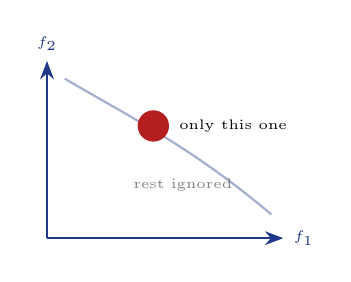
\begin{tikzpicture}[scale=0.75]
      \draw[-{Stealth}, NavyBlue, thick] (0,0)--(4,0) node[right,font=\tiny]{$f_1$};
      \draw[-{Stealth}, NavyBlue, thick] (0,0)--(0,3) node[above,font=\tiny]{$f_2$};
      \draw[NavyBlue!40, thick]
            (0.3,2.7) .. controls (1.5,2.0) and (2.5,1.5) .. (3.8,0.4);
      % Only one result
      \node[circle, fill=AlertRed, inner sep=4pt,
            label={[font=\tiny]right:only this one}] at (1.8,1.9) {};
      \node[font=\tiny, text=gray] at (2.3,0.9) {rest ignored};
    \end{tikzpicture}
    \end{center}
    \small They require you to \emph{decide} on a weighting up front.
    If priorities change, you must re-run from scratch.

    \column{0.48\textwidth}
    \textbf{EAs naturally find \emph{many} solutions}
    \begin{center}
    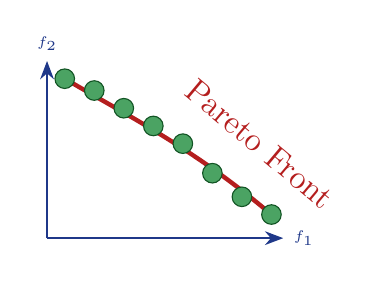
\begin{tikzpicture}[scale=0.75]
      \draw[-{Stealth}, NavyBlue, thick] (0,0)--(4,0) node[right,font=\tiny]{$f_1$};
      \draw[-{Stealth}, NavyBlue, thick] (0,0)--(0,3) node[above,font=\tiny]{$f_2$};
      \draw[AlertRed, ultra thick]
            (0.3,2.7) .. controls (1.5,2.0) and (2.5,1.5) .. (3.8,0.4);
      \node[font=\large, text=AlertRed, rotate=-40] at (3.6,1.6) {Pareto Front};
      \foreach \x/\y in {0.3/2.7, 0.8/2.5, 1.3/2.2, 1.8/1.9,
                          2.3/1.6, 2.8/1.1, 3.3/0.7, 3.8/0.4}
        \node[circle, fill=GreenOK!80, draw=GreenOK!60!black, inner sep=2.5pt]
              at (\x,\y) {};
    \end{tikzpicture}
    \end{center}
    \small The \textbf{population} maps naturally to a \emph{set} of trade-off solutions.
    One run gives the full picture.
  \end{columns}

  \vspace{0.4em}
  \begin{center}
    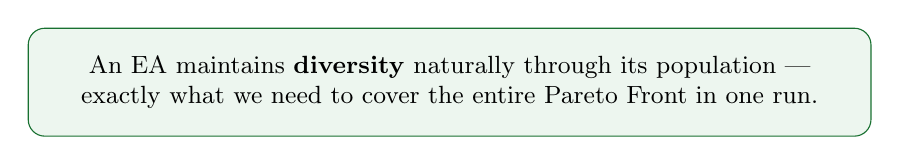
\begin{tikzpicture}
      \node[draw=GreenOK!80!black, fill=GreenOK!8, rounded corners=6pt,
            font=\small, inner sep=10pt, text width=10cm, text centered]
        {An EA maintains \textbf{diversity} naturally through its population
         — exactly what we need to cover the entire Pareto Front in one run.};
    \end{tikzpicture}
  \end{center}
\end{frame}


%% ============================================================
%% SLIDE 11 — Transition to MOEA/D
%% ============================================================
% \begin{frame}{So\ldots\ Where Does MOEA/D Come In?}

%   \begin{center}
%   \begin{tikzpicture}[
%     box/.style={draw=NavyBlue, fill=NavyBlue!10, rounded corners=8pt,
%                 minimum width=4.0cm, minimum height=1.4cm,
%                 align=center, font=\small\bfseries, text=NavyBlue,
%                 inner sep=8pt},
%     plus/.style={font=\Large\bfseries, NavyBlue},
%     result/.style={draw=GreenOK!80!black, fill=GreenOK!10, rounded corners=8pt,
%                    minimum width=9.5cm, minimum height=1.5cm,
%                    align=center, font=\bfseries, text=GreenOK!60!black,
%                    inner sep=10pt}
%   ]

%     \node[box] (ea)  at (-2.8, 0.5) {Evolutionary\\Algorithm\\(what we just learned)};
%     \node[plus]      at ( 0.0, 0.5) {$+$};
%     \node[box] (dec) at ( 2.8, 0.5)
%           {Decomposition\\(split the problem into\\many smaller sub-problems)};

%     \node[result] at (0, -1.6)
%           {MOEA/D — Solves all sub-problems simultaneously using the EA loop};

%     \draw[-{Stealth[length=6pt]}, GreenOK!70!black, thick]
%           (ea.south)  .. controls +(0,-0.6) and +(-2,0) .. (-1.2,-1.0);
%     \draw[-{Stealth[length=6pt]}, GreenOK!70!black, thick]
%           (dec.south) .. controls +(0,-0.6) and +( 2,0) .. ( 1.2,-1.0);
%   \end{tikzpicture}
%   \end{center}

%   \vspace{0.3em}

%   \begin{columns}[T]
%     \column{0.48\textwidth}
%     \textbf{What you now understand:}
%     \begin{itemize}
%       \item Solutions are candidates that get scored
%       \item Selection, crossover, mutation drive improvement
%       \item A population naturally explores many trade-offs
%     \end{itemize}

%     \column{0.48\textwidth}
%     \textbf{What MOEA/D adds:}
%     \begin{itemize}
%       \item Each solution ``owns'' a direction in objective space
%       \item Neighbouring solutions help each other improve
%       \item This makes the search much more \textbf{structured and efficient}
%     \end{itemize}
%   \end{columns}

%   \vspace{0.4em}
%   \begin{center}
%     \begin{tikzpicture}
%       \node[draw=NavyBlue!50, fill=NavyBlue!5, rounded corners=5pt,
%             font=\small\itshape, inner sep=8pt, text width=9.5cm, text centered]
%         {``Decompose the multi-objective problem into many scalar
%           sub-problems and solve them simultaneously.''\\[0.3em]
%          \normalfont\scriptsize --- Zhang \& Li, 2007};
%     \end{tikzpicture}
%   \end{center}
% \end{frame}

\end{document}